\documentclass[a4paper, 12pt]{article}
\usepackage[utf8]{inputenc}

\usepackage[margin=1.2in]{geometry}
\usepackage{natbib}
\usepackage{graphicx}
\usepackage{placeins}
\usepackage{caption}
\newcommand\tab[1][1cm]{\hspace*{#1}}
\geometry{top = 1in}
\setlength{\textfloatsep}{1\baselineskip plus 0.2\baselineskip minus 0.5\baselineskip}
\renewcommand\textfraction{.1}


\title{Análisis Exploratorio de Datos \\ Trabajo Práctico 1 - Organización de Datos}
\author{Nombre de grupo}
\date{Poner fecha}

\begin{document}
\begin{figure}
    \centering
    \makebox[\textwidth]{
\includegraphics[width=250pt]{logofiuba.jpg}}
\end{figure}

\maketitle

\FloatBarrier
\begin{center}
        \begin{tabular}{ |c|c|c| }
          \hline
          Nombre & Padrón & Mail \\
          \hline\hline
          Álvarez, Federico & 99266 & fede.alvarez1997@gmail.com \\
          \hline
          La Torre, Gabriel & 87796 & latorregab@gmail.com \\
          \hline
          Medrano, Lucas Nicolás & 99247 & lucasmedrano97@gmail.com \\
          \hline
          Piro Martino, Ariel & 99469 & ariel.piro@hotmail.com \\
          \hline
        \end{tabular}
\end{center}
\FloatBarrier

\newpage

\tableofcontents
\newpage
\section{Introduction}
	\tab En el trabajo se hace un análisis exploratorio de un set de datos provistos por la empresa Jampp. En el mismo se encuentra información de subastas, instalaciones, clicks, entre otros.\\
	\tab Primero se hará una visión general de los archivos (installs.csv, clicks.csv, auctions.csv, events.csv) para entender la distribución y la cantidad de datos, el significado de las columnas, reconocer las columnas que no aportan información (por ejemplo, las que tienen todos sus valores nulos), reconocer el tipo de datos en cada columna, seguido de un análisis mas profundo para obtener mas información de los datos. Luego se hará un análisis global, buscando información relativa a los archivos en conjunto, permitiendo obtener otro tipo de información.

\section{Análisis individual de archivos}
\subsection{Subastas}
	\subsubsection{Análisis general} \label{analisis general}
	 \tab El archivo 'auctions.csv' contiene información acerca de subastas.
	Hay dos columnas que no nos aportan información significante. 'auction\_type\_id' tiene todos sus valores 		nulos, por lo que no fue tomada en cuenta para el análisis. 'country' informa un solo valor posible, que se supone que debe ser Argentina.
	\tab La columna platforms tiene dos valores posibles (1 y 2) que se supone son Android e iOS. Va a ser importante para el análisis que hagamos más adelante. De ahora en más, platform y sistema operativo serán sinónimos en este informe.
	\tab Por último, 'source' nos da información acerca del exchange de donde surge la subasta.
	\tab Además vemos que ningún valor de este archivo, excluyendo la columna 'auction\_type\_id', es nulo, por lo que no es necesario tomar ninguna decisión respecto a eso.
	
	\subsubsection{Subastas por día de Marzo}
	\tab Como primer acercamiento a este set de datos, es interesante ver cómo se distribuye la cantidad de subastas en los días que incluye el archivo (05/03/19 al 13/03/19). El gráfico \ref{subastasmarzo} representa dicha distribución. En él se pueden observar varias cosas:
	\begin{itemize}
		\item La cantidad de subastas parece, en general, aumentar con el paso de los dias.
		\item El valor del último día es mas del doble del valor del primer día.
		\item El mayor aumento se da del sexto al septimo día.
		\item La cantidad de subastas varía entre unos valores extremos, aproximados, de un millón y 3 millones.
	\end{itemize}

	\FloatBarrier
		\begin{figure}
			\centering
			   	\makebox[\textwidth]{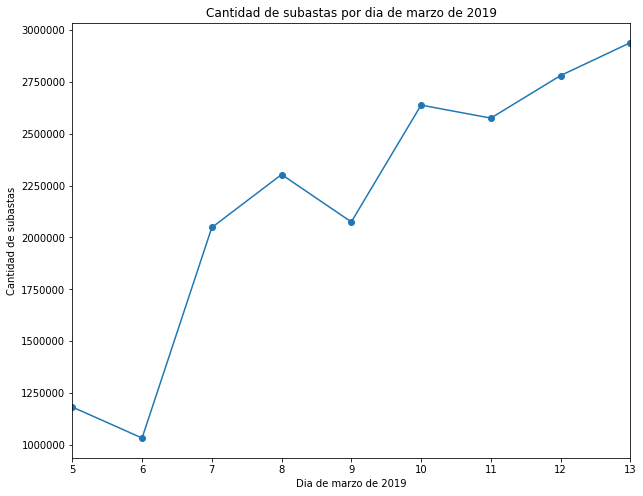
\includegraphics[width=300pt]{images/auctions/subastaspordia.png}}
		   		\caption{Cantidad de subastas por día de Marzo}
			   	\label{subastasmarzo}
		\end{figure}
	\FloatBarrier
			
	\subsubsection{Subastas por día de Marzo por sistema operativo}
	\tab Otro punto interesante es dividir el problema. Obtener la distribución de subastas en los días con datos disponibles para cada plataforma (Android e iOS). En la imagen \ref{subastasmarzoSO} se pueden observar las cantidades. Observese que llamamos '1' y '2' a las plataformas, ya que no sabemos cuál es Android y cuál es iOS.
	\tab Puntos interesantes a reconocer:
	
	\begin{itemize}
		\item La cantidad de subastas para la plataforma '1' es, salvo en el cuarto y el quinto día, considerablemente mayor a la cantidad para la plataforma '2'.
		\item La figura de la plataforma '2' es mucho mas "chata" que la de la plataforma '1', la cual representa mas picos y saltos.
		\item La figura de la plataforma '1' es muy parecida a la del gráfico \ref{subastasmarzo}, mientras que la de la plataforma '2' no lo es. Esto es resultado, principalmente, de lo indicado en el primer ítem. Este análisis puede llegar a ser muy útil para reconocer partes de los datos que son representativas del total.
	\end{itemize}
	
	\FloatBarrier	
	\begin{figure}
			\centering
	   		\makebox[\textwidth]{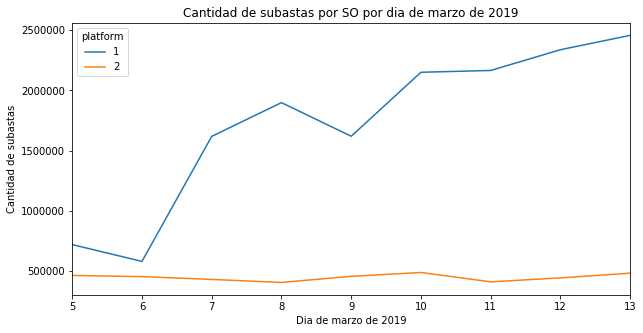
\includegraphics[width=350pt]{images/auctions/subastaspordiaSO.png}}
		   	\caption{Cantidad de subastas por día de Marzo y por sistema operativo}
		   	\label{subastasmarzoSO}
		\end{figure}
	\FloatBarrier
			
	\subsubsection{Subastas por hora del día}
	\tab Ahora vamos a analizar cómo se distribuyen las subastas a lo largo del día. Para esto hacemos un gráfico de hora del día contra cantidad de subastas (Gráfico \ref{subastashora}).\newline
	\tab Desde un análisis cualitativo se pueden observar algunos puntos:
	\begin{itemize}
		\item Parece ser que la mayor cantidad de subastas se distribuyen por la noche y la madrugada.
		\item La cantidad de subastas es poca en horas de la mañana y el mediodía. En el gráfico se puede ver un gran valle en esa parte del día.
	\end{itemize}
	
	\FloatBarrier
		\begin{figure}
			\centering
			\makebox[\textwidth]{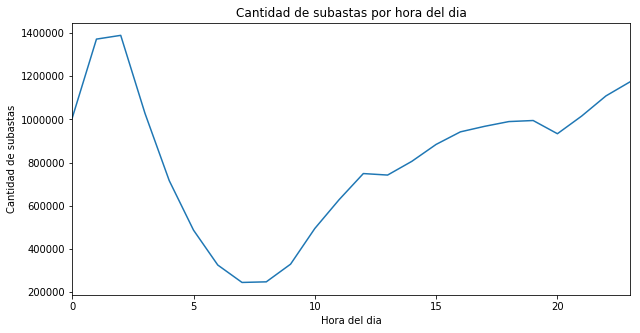
\includegraphics[width=350pt, bb=0 0 640 480]{images/auctions/subastasporhora.png}}
		   	\caption{Cantidad de subastas por hora del día}
			\label{subastashora}
		\end{figure}
	\FloatBarrier
	\subsubsection{Subastas por hora del día por sistema operativo}
	\tab Al igual que se hizo antes, podemos dividir el gráfico para ambas plataformas. Vemos que pasa algo muy parecido que lo que pasaba para la cantidad de subastas por día. El gráfico de la plataforma '1', al tener una cantidad mucho mayor de subastas, es la que predomina en el gráfico de la sección "Subastas por hora del día", y por eso sus gráficos son tan parecidos. EL gráfico de la plataforma '2' es bastante mas chato, y con cantidades de subastas mucho mas chicas.

	\FloatBarrier
		\begin{figure}
			\centering
			\makebox[\textwidth]{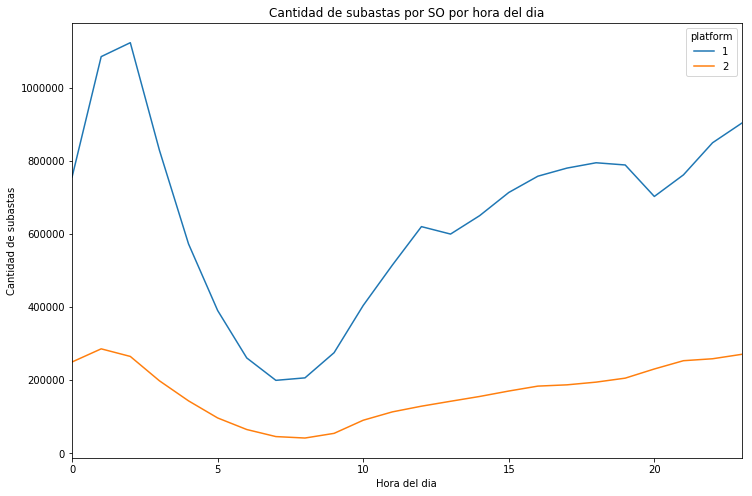
\includegraphics[width=220pt]{images/auctions/subastasporhoraS0.png}}
		   	\caption{Cantidad de subastas por hora del día por sistema operativo}
			\label{subastashoraSO}
		\end{figure}
	\FloatBarrier	
	
	\subsubsection{Subastas por sistema operativo}
	\tab Resulta interesante conocer cuál es el sistema operativo para el cual se generan más subastas. Es algo que ya se venía viendo en la forma y nivel (cantidad de subastas) de los gráficos anteriores. Sin embargo, los gráficos vistos hasta ahora no dan un conocimiento directo de la relacion de las cantidades de subastas de ambas plataformas. 
	\tab En las figuras que se ven a continuación podemos confirmar que lo que indicabamos en los gráficos anteriores era cierto. La cantidad de subastas es mucho mayor para la plataforma '1'. Además, ahora tenemos una visión mas cuantitativa de esta relación (en la imagen \ref{subastasSOporcentajes} vemos una relación porcentual, mientras que la imagen \ref{subastasSOcantidades} nos da mas idea de las cantidades).
	
	\FloatBarrier
		\begin{figure}
			\centering
			\makebox[\textwidth]{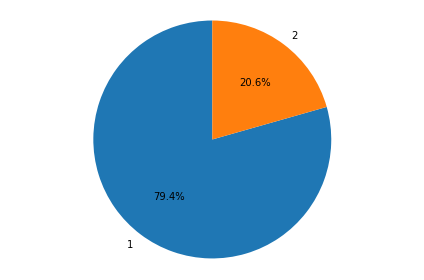
\includegraphics[width=350pt]{images/auctions/subastasporSO.png}}
		   	\caption{Porcentaje de subastas para cada plataforma}
			\label{subastasSOporcentajes}
		\end{figure}
	\FloatBarrier
	
	\FloatBarrier
		\begin{figure}
			\centering
			\makebox[\textwidth]{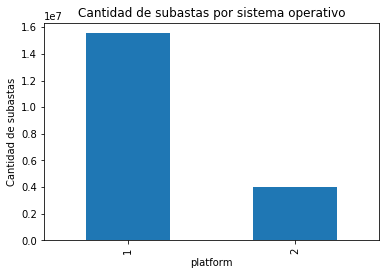
\includegraphics[width=350pt]{images/auctions/subastasporSOcantidad.png}}
		   	\caption{Porcentaje de subastas para cada plataforma}
			\label{subastasSOcantidades}
		\end{figure}
	\FloatBarrier	
	
	\subsubsection{Subastas por source}
	\tab Como indica la introducción a esta sección (vease \ref{analisis general}), source nos indica el exchange que generó la subasta. Se puede obtener, a partir de los datos, cuáles son los exchanges principales, y cuántas subastas generan.
	\tab A tener en cuenta:
	\begin{itemize}
		\item Los que se muestran son todos los exchanges que aparecen en el archivo.
		\item Al igual que en las plataformas, los exchanges se toman por un id, y no por su nombre.
		\item Hay una clara diferencia en las cantidades.
		\begin{itemize}
			\item El exchange '0' es predominante, superando ampliamente el millon de subastas generadas.
			\item El siguiente (source '1') aunque es mucho menor que el '0', sigue superando a los demas exchange por una gran cantidad. Llegando a las 400000 subastas generadas
			\item Los exchanges '2', '5' y '6' parecen no tener mucho peso en el gráfico. Aunque quizás podría tomarse la cantidad del '5' como significativa.
		\end{itemize}  
	\end{itemize}
	
	\FloatBarrier
		\begin{figure}
			\centering
			\makebox[\textwidth]{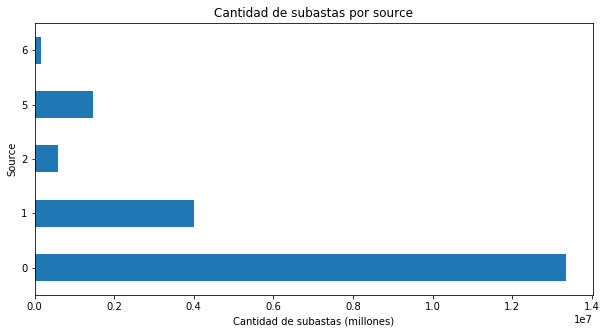
\includegraphics[width=\textwidth]{images/auctions/subastasporsource.png}}
		   	\caption{Cantidad de subastas para cada source}
			\label{subastassource}
		\end{figure}
	\FloatBarrier
	
	\subsubsection{Análisis de los dispositivos en las subastas}
	\tab Otro punto a analizar son los dispositivos. Es un punto que trajo un problema al analizar los datos, y que puede cambiar la forma en la que se entienden los datos anteriormente mencionados.
	Podemos, por ejemplo, ver el top diez de dispositivos de los cuales se generan mas subastas.
	\FloatBarrier
		\begin{figure}
			\centering
			\makebox[\textwidth]{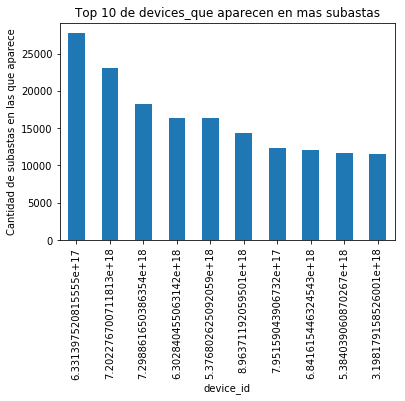
\includegraphics[width=350pt]{images/auctions/top10devicessubastas.png}}
		   	\caption{Top 10 de dispositivos con mayor cantidad de subastas}
			\label{top10devicessubastas}
		\end{figure}
	\FloatBarrier
	
	\tab Ahora el problema.\newline
	\tab En total, en las 19571319 subastas, aparecen 206171 dispositivos. Algo interesante sería conocer cuántos tienen cada plataforma. Por lo que hacemos un gráfico.
	
	\FloatBarrier
		\begin{figure}
			\centering
			\makebox[\textwidth]{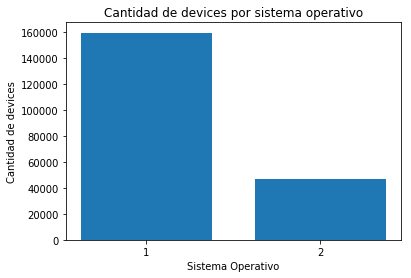
\includegraphics[width=350pt]{images/auctions/devicesporSO.png}}
		   	\caption{Cantidad de dispositivos para cada plataforma}
			\label{devicesporSO}
		\end{figure}
	\FloatBarrier
	
	\tab Al obtener los datos del gráfico, observamos que la suma de las cantidades de dispositivos para cada plataforma es 206453. ¡Esto es mayor a la cantidad total de dispositivos (206171)!\newline
	\tab La causa de este problema se entiende al conocer cómo se obtuvieron las cantidades. Primero se contó la cantidad de dispositivos total. Luego se separaron los que tuvieran plataforma '1' de los que tuvieran plataforma '2' (tener en cuenta que como hay una fila por subasta, cada dispositivo puede aparecer en filas distintas). Al sumar ambas cantidades obtenemos un número mayor que el total, por lo que es evidente que hay dispositivos que tienen ambas plataformas, es decir, en algunas filas aparecen con un valor de la columna 'platform' y en otras filas con otro.
	
	\tab Haciendo una simple resta, se puede ver que la cantidad de dispositivos que aparecen con plataformas distintas es 282, y que en total participan en 47862 subastas. De hecho hay un dispositivo (5.292967062497395e+18) que aparece en el top 300 de cantidad de subastas.
	
	\tab Esto puede alterar los análisis que incluyen división en plataformas. Sin embargo, no es trivial que haya que borrar estos datos, porque se estarían borrando casi 50000 subastas. Además, dejar los datos como están no altera a los estudios que se hagan sin dividir el problea por sistemas operativos. Por lo tanto se decidió dejar los datos, y saber que el análisis que se hace cuando se divide el problema, puede no ser tan preciso.
	

\subsection{Clicks}

\subsection{Eventos}

\subsection{Instalaciones}
	\subsubsection{Introducción}
		Los datos sobre instalaciones fueron provistos por Jampp en el archivo \texttt{installs.csv}, el cual contenía información acerca de todas las instalaciones registradas entre los días 5 y 13  Marzo del corriente año, indicando el tipo de aplicaciones descargadas, su fecha de descarga, país de origen, modelo, marca e idioma del dispositivo, entre otras cosas. 
	
		Cabe destacar que se descartaron datos como las direcciones ip y los varios id únicos generados para cada instalación, puesto que no aportaban información relevante al análisis que se pretende hacer en este trabajo, como también los datos del \textit{session user agent}, ya que la misma empresa informó que no los consideran de importancia y pudieron haberse visto modificados por los propios agentes que les proveyeron los datos.
	
	\subsubsection{Instalaciones por día y hora}
		Para comenzar, lo primero que haremos será ver cómo se distribuyen las instalaciones en el periodo dado. 
		\FloatBarrier
		\begin{figure}[h]
			\centering
			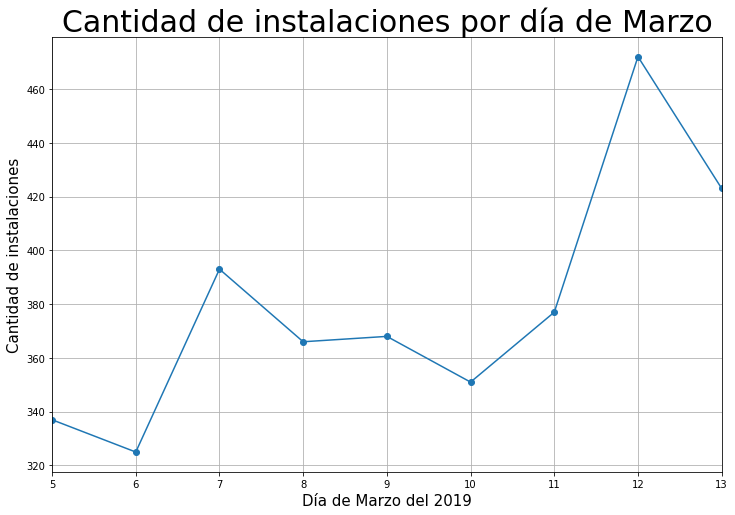
\includegraphics[width=\textwidth]{images/installs/installspordia.png}
			\caption{Instalaciones por día de Marzo}
		\end{figure}
		\FloatBarrier
		
		Como se puede observar, se registran ascensos considerables entre los días 6 y 7 y 11 y 12, con respectivas caídas al día siguiente, pero manteniendo una tendencia general al alza.
		
		\FloatBarrier
		\begin{figure}[h]
			\centering
			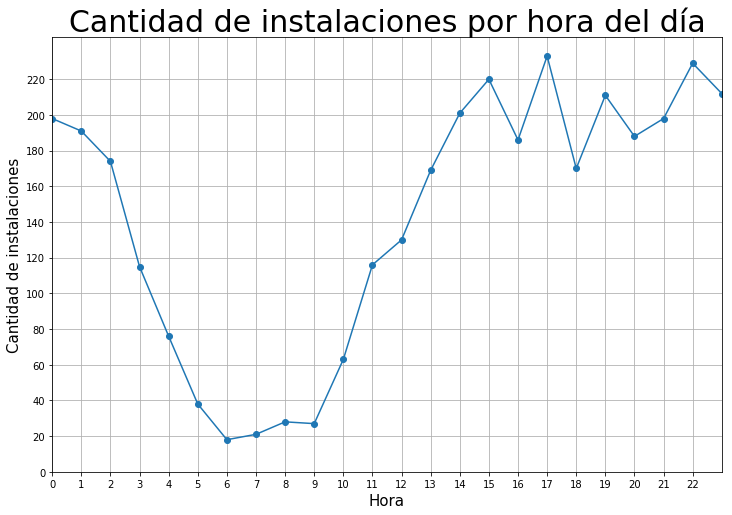
\includegraphics[width=\textwidth]{images/installs/installsxhora.png}
			\caption{Instalaciones por hora del día}
		\end{figure}
		\FloatBarrier
		
		 El gráfico anterior nos indica que la gran mayoría de las instalaciones se registran en horas de la tarde y la noche, con un pico a las 5 de la tarde. Cabe destacar a su vez el notorio valle que se da en horas de la mañana, donde el número es hasta diez veces menor que en el punto máximo.
		 
		 Para un análisis más general, la siguiente figura engloba los dos puntos mencionados anteriormente.
		 
		\FloatBarrier
		\begin{figure}[h]
			\centering
			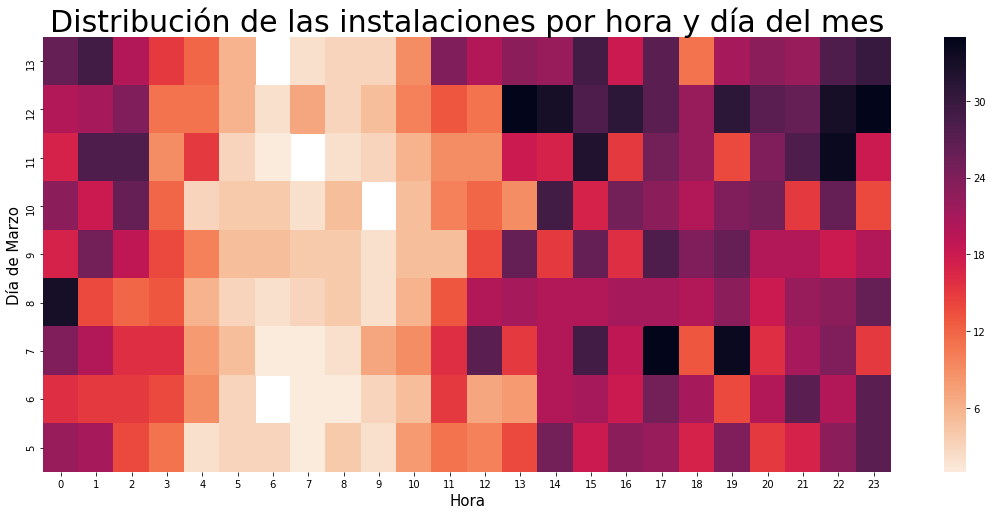
\includegraphics[width=\textwidth]{images/installs/heatmapfecha.png}
			\caption{Instalaciones por fecha y hora}
		\end{figure}
		\FloatBarrier
		
		Se puede observar claramente el valle de las horas de la mañana, como así también el pico que se da en el día 12. Sin embargo, este gráfico resulta útil ya que permite notar que tanto en los días 6 y 13 a las 6 de la mañana, el día 11 a las 7 y el 10 a las 9 no se produjo ninguna instalación.
		
	\subsubsection{Instalaciones por aplicación} \label{aplicaciones}
		Resultará de utilidad conocer de que aplicación provienen las instalaciones registradas y observar cual es la tendencia en ese aspecto para determinar en cuales es mejor colocar la publicidad.
		
		\FloatBarrier
		\begin{figure}[h]
			\centering
			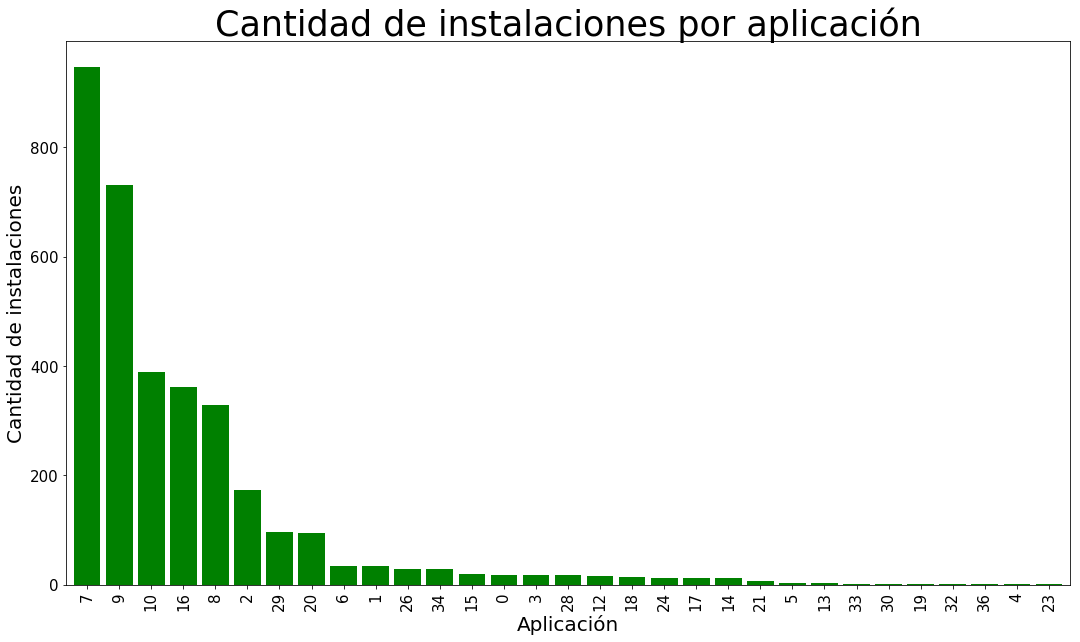
\includegraphics[width = \textwidth]{images/installs/aplicacionesvc.png}
			\caption{Instalaciones por aplicación}
		\end{figure}
		\FloatBarrier
		
		La figura anterior muestra un dominio claro de las aplicaciones 7 y 9 por sobre las demás, ya que la segunda casi duplica en cantidad a la tercera. Además, se puede ver otra diferencia importante{\textemdash}otra vez, de casi el doble{\textemdash}entre la quinta y la sexta, lo que deja en evidencia cuales son las que dominan en este campo, puesto que las primeras cinco aplicaciones concentran más del 80\% de las instalaciones.
		
	\subsubsection{Instalaciones por fecha según la aplicación}
		A continuación veremos a qué aplicaciones pertenecen las instalaciones según el día y la hora del día, lo que puede servir para determinar en qué momento apostar por una u otra aplicación. Cabe destacar que, para ello se agruparon todas aquellas aplicaciones que generaron un número muy bajo (menos de 90) de instalaciones en la categoría \textit{other}.
		
		\FloatBarrier
		\begin{figure}[h]
			\centering
			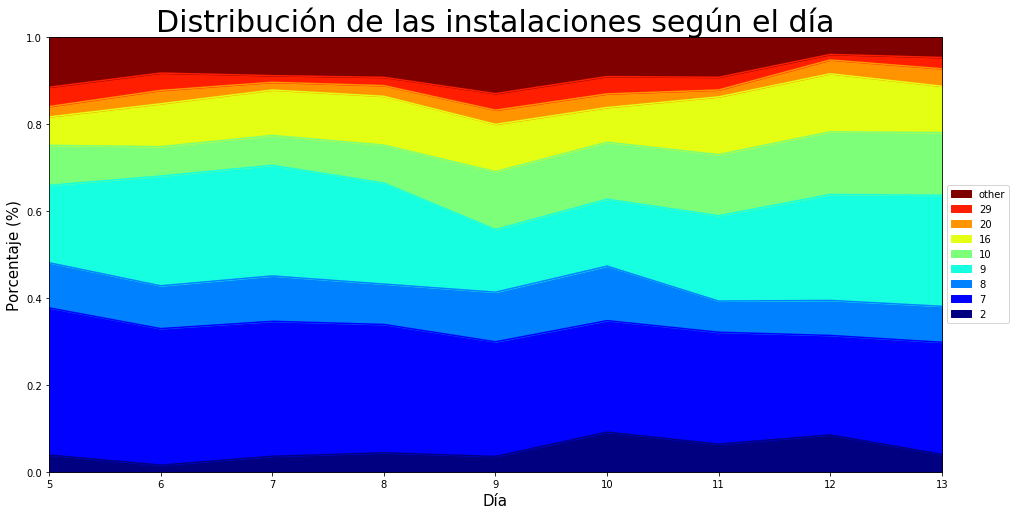
\includegraphics[width= \textwidth]{images/installs/appsxdiaarea.png}
			\caption{Incidencia de las aplicaciones según el día}
		\end{figure}
		\FloatBarrier
		
		Como se puede observar, la aplicación 7 dominó la mayoría de los días aunque disminuyendo hacia el 12 y el 13, donde fue superada por la 9. La tercera aplicación con más instalaciones, la 10, se mantuvo bastante estable durante los últimos cinco días, mientras que los días 10 y 12 la número 2, de poca preponderancia en otros días, obtuvo su mejor resultado. Cabe aclarar además, que si bien en días como el 9 se ve bastante incidencia de la categoría \textit{other}, ésta engloba los resultados de 23 aplicaciones distintas.
		
		\FloatBarrier
		\begin{figure}[h]
			\centering
			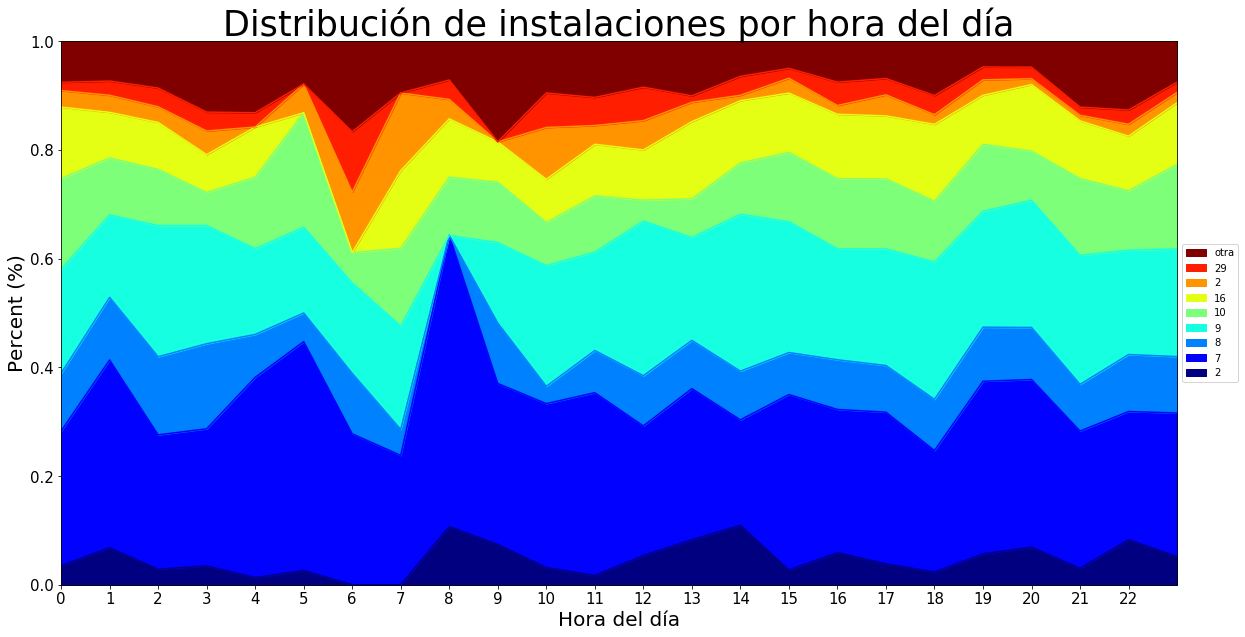
\includegraphics[width=\textwidth]{images/installs/appsxhora.png}
			\caption{Incidencia de las aplicaciones según la hora del día}
		\end{figure}
		\FloatBarrier
		
		En cuanto a la hora cabe destacar que la segunda aplicación en instalaciones no tiene presencia alguna a las 8 a.m., que es a su vez el momento del día donde más incidencia tiene una aplicación de poca presencia como la 2. La tendencia sigue mostrando a la número 7 como dominadora absoluta en todos los horarios.
		
	\subsubsection{Instalaciones por país}
		El país de origen es un aspecto a considerar a la hora de decidir qué advertisers priorizar para cada situación. En este caso Jampp nos provee información de instalaciones en dos países distintos.
		
		\FloatBarrier
		\begin{figure}[h]
			\centering
			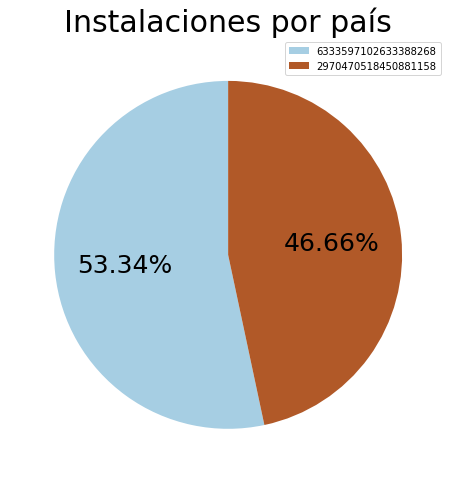
\includegraphics[width=200pt]{images/installs/piechartpaises.png}
			\caption{País de origen de las instalaciones}
		\end{figure}
		\FloatBarrier
		
		La proporción es bastante pareja, con leve mayoría para el país \texttt{6333597102633388268}.
		
	\subsubsection{Instalaciones por tipo}
		Los dispositivos se clasifican en dos grandes grupos, aquellos que provienen de Apple y los que provienen de Google.
		
		\FloatBarrier
		\begin{figure}[h]
			\centering
			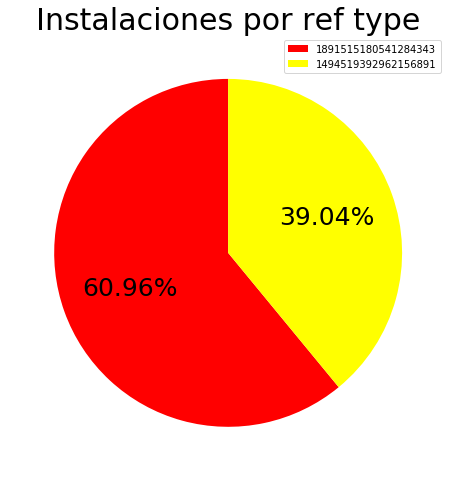
\includegraphics[width= 200pt]{images/installs/ref_type.png}
			\caption{Tipo de referencia de las instalaciones}
		\end{figure}
		\FloatBarrier
		
		Como se observa, el claro dominador es \texttt{1891515180541284343}.
		
	\subsubsection{Aplicaciones por país y tipo}
	
		Analicemos ahora de donde provienen las instalaciones de las 5 aplicaciones con más installs.
	
		\FloatBarrier
		\begin{figure}[h]
			\centering
			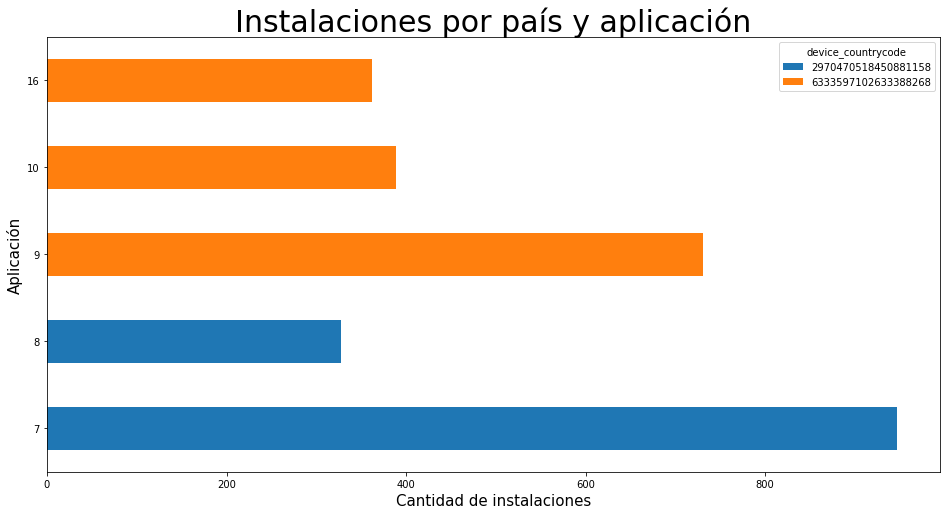
\includegraphics[width=\textwidth]{images/installs/appsxpais.png}
			\caption{Distribución de países para las top 5 aplicaciones en instalaciones}
		\end{figure}
		\FloatBarrier
		
		Sorprendentemente el gráfico es determinante, las aplicaciones provienen o de un país o del otro, ninguna está presente en ambos.
		
		\FloatBarrier
		\begin{figure}[h]
			\centering
			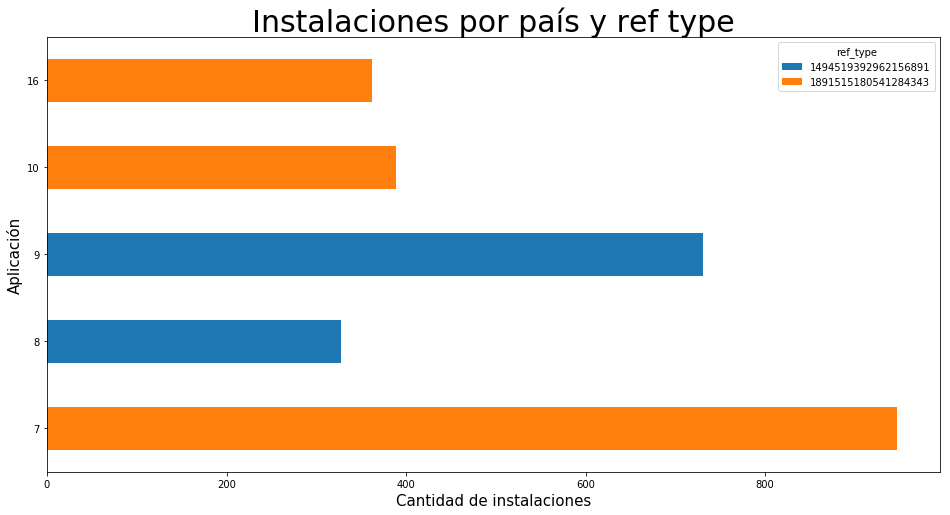
\includegraphics[width=\textwidth]{images/installs/paisref.png}
			\caption{Distribución de ref types para las top 5 aplicaciones en instalaciones}
		\end{figure}
		\FloatBarrier
		
		En el caso de los tipos sucede lo mismo, aunque esto es más esperable, ya que existen muchas aplicaciones que son exclusivas de Apple o de Google. Esta información es útil a la hora de determinar el advertiser a seleccionar en cada subasta, ya que la aplicación o servicio a mostrar en la publicidad debe estar disponible para ese tipo.
	
	\subsubsection{Idiomas y aplicaciones}
		Otro aspecto importante a considerar será el idioma del dispositivo al que se le mostrará la publicidad, ya que el usuario debe entender el mensaje. 
		
		\FloatBarrier
		\begin{figure}[h]
			\centering
			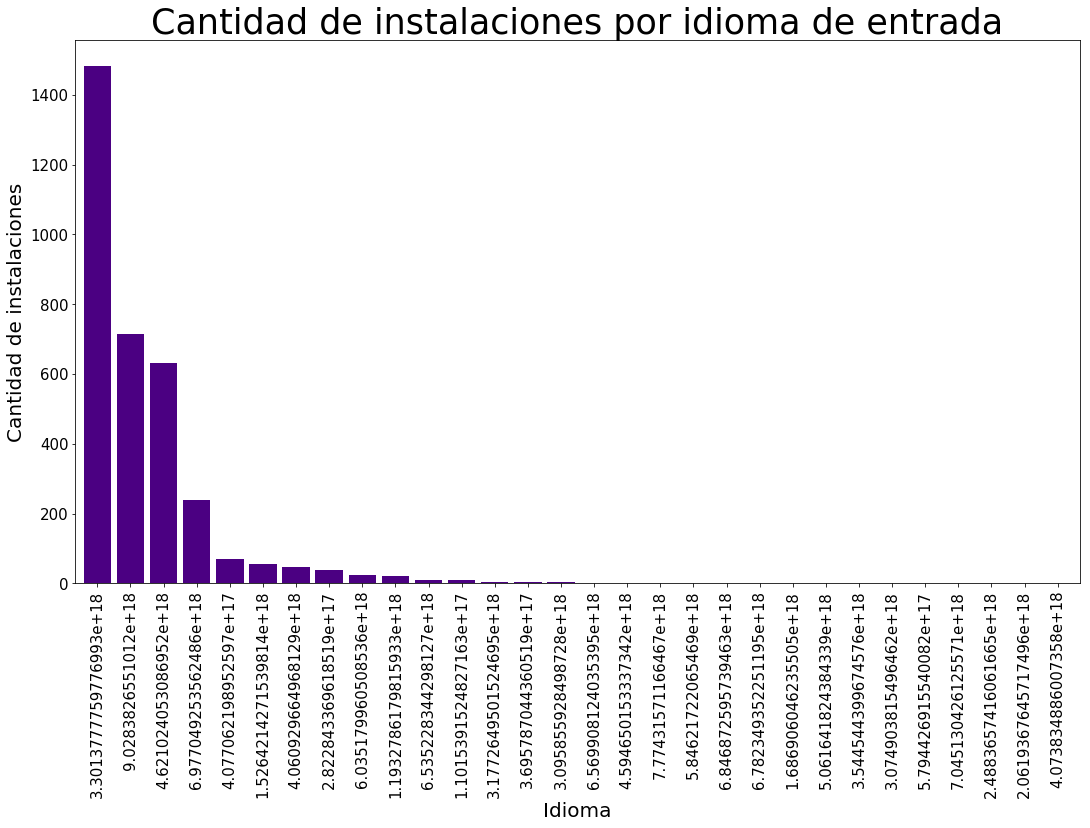
\includegraphics[width=\textwidth]{images/installs/idiomas.png}
			\caption{Idioma de entrada con mayor número de instalaciones}
		\end{figure}
		\FloatBarrier
		
		Vemos que hay un idioma claramente predominante, luego dos en nivel parejo y una brecha considerable.
		Por esta razón, y para mayor simplicidad de los gráficos, se agruparán los 26 idiomas menos predominantes en la categoría \textit{other}. 
		
		Analicemos ahora como se distribuyen los idiomas en las 5 applicaciones más instaladas.
		
		\FloatBarrier
		\begin{figure}[h]
			\centering
			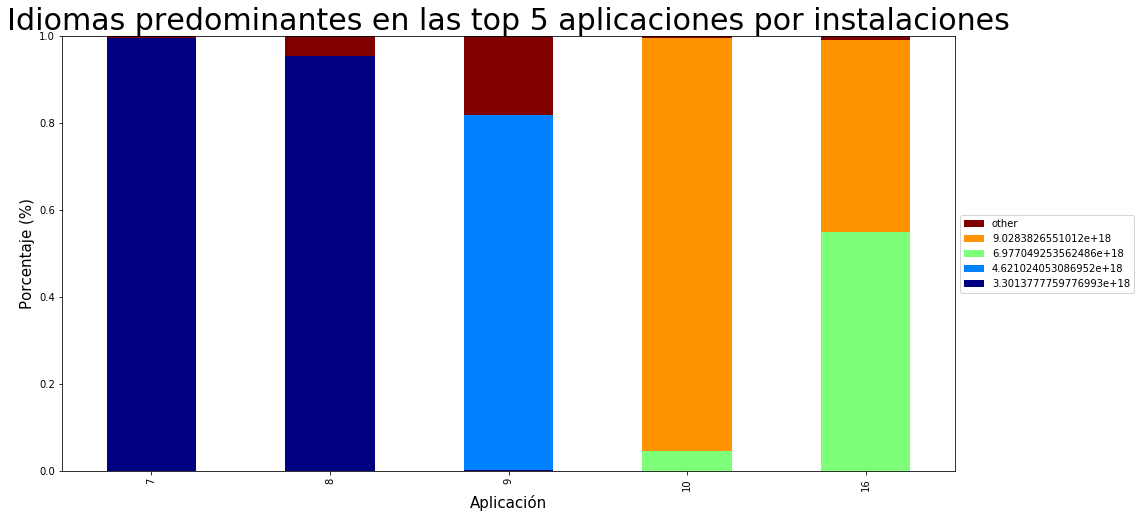
\includegraphics[width=\textwidth]{images/installs/idiomasapps.png}
			\caption{Idioma de entrada de los dispositivos para las 5 aplicaciones líderes en instalaciones}
		\end{figure}
		\FloatBarrier
		
		Como se puede ver, las aplicaciones líderes (7 y 9 respectivamente) se utilizan con idiomas distintos, mientras que en 10 y 16 predominan otros dos lenguajes diferentes.
		
	\subsubsection{Instalaciones wifi y user agents}
	
		Otro aspecto a considerar es la conexión con la que cuentan los usuarios al momento de decidir si hacer caso o no a alguna publicidad. Los datos que nos proporciona Jampp nos indican si las instalaciones fueron hechas vía conexión wifi.
		
		Inicialmente se esperaría que sea mayor el número de instalaciones vía wifi, ya que los datos móviles suelen tener un límite de uso bastante bajo.
		
		\FloatBarrier
		\begin{figure}[h]
			\centering
			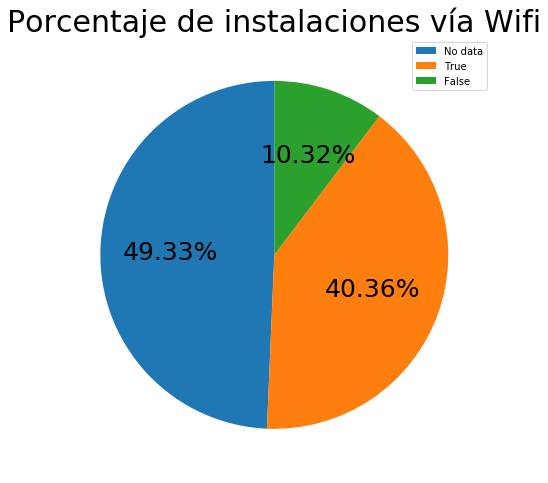
\includegraphics[width=200pt]{images/installs/Wifi.png}
			\caption{Instalaciones por conexión wifi.}
		\end{figure}
		\FloatBarrier
		
		Sorprendentemente la figura muestra que para una gran mayoría de las instalaciones no se proporcionó data respecto de la conexión. Sin embargo, y en concordancia con lo mencionado previamente, en los casos en los que sí se tiene información resulta claro ver que la mayor parte de dichas instalaciones sí fueron realizadas vía conexión wifi. 
		
		Trasladando estos datos a las aplicaciones vemos.
		
		\FloatBarrier
		\begin{figure}[h]
			\centering
			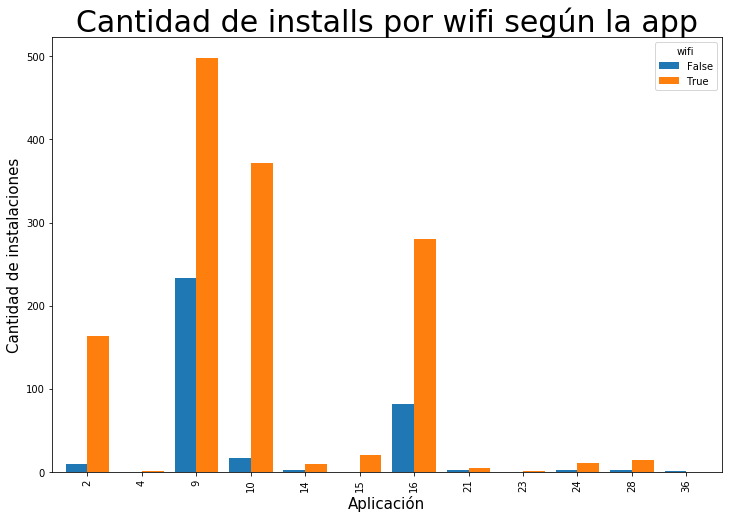
\includegraphics[width=\textwidth]{images/installs/appswifi.png}
			\caption{Instalaciones por conexión wifi según la aplicación.}
		\end{figure}
		\FloatBarrier
		
		Lo primero que observamos es que la cantidad de aplicaciones de las que se tienen datos de conexión es reducida en comparación al total, ya que , por ejemplo, la aplicación líder en instalaciones no especifica tipo de conexión en ninguna de sus installs. Sin embargo, de este gráfico puede tomarse el hecho de que, si bien la tendencia indica que la mayoría de las instalaciones de las que se tienen datos se realizaron vía wifi, hay aplicaciones como 21 ,donde la proporción es más pareja, o la 36, donde se invierte. Esto puede servir para determinar qué tipo de publicidad mostrar, puesto que en los casos donde no se cuenta con wifi hay que tener en cuenta el consumo, para no gastarle los datos al usuario.
		
		Por otra parte, el hecho de que un install se haya realizado por wifi nos permite conocer otro dato importante, el \textit{user agent} relacionado a la acción. 
		
		Análogamente a lo hecho al comienzo de la sección \ref{aplicaciones}, se analizaron los user agents.
		
		\FloatBarrier
		\begin{figure}[h]
			\centering
			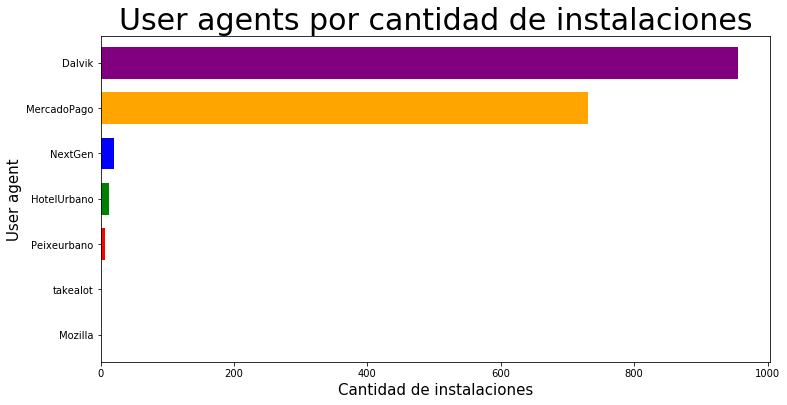
\includegraphics[width=\textwidth]{images/installs/useragents.png}
			\caption{User agents por instalaciones}
		\end{figure}
		\FloatBarrier
		
		Resulta evidente que los dominadores absolutos de la categoría son Dalvik y MercadoPago, con agentes casi sin presencia, como Mozilla y takealot, que cuentan sólamente con una instalación.
		
		\subsubsection{Instalaciones atribuidas a Jampp}
		Será de particular importancia saber cuantas de las instalaciones se le atribuyeron oficialmente a Jampp, es decir, cuantas de ellas fueron realmente obra de la empresa. Los datos proporcionados hacen dos tipos de distinciones.
		
		\FloatBarrier
		\begin{itemize}
		\item \textbf{Attributed}: Indica si la instalación le fue reconocida oficialmente a Jampp.
		\item \textbf{Implicit}: Indica si la instalación se registró de manera implícita, es decir, le fue atribuida a una empresa de la competencia.
		\end{itemize}
		\FloatBarrier
		
		En este aspecto, los datos indican que absolutamente ninguna de las instalaciones le fue atribuida a Jampp, lo que indica un porcentaje de efectividad del 0\%. Sin embargo, para la categoría \textit{implicit}, los resultados fueron los siguientes.
		
		\FloatBarrier
		\begin{figure}[h]
			\centering
			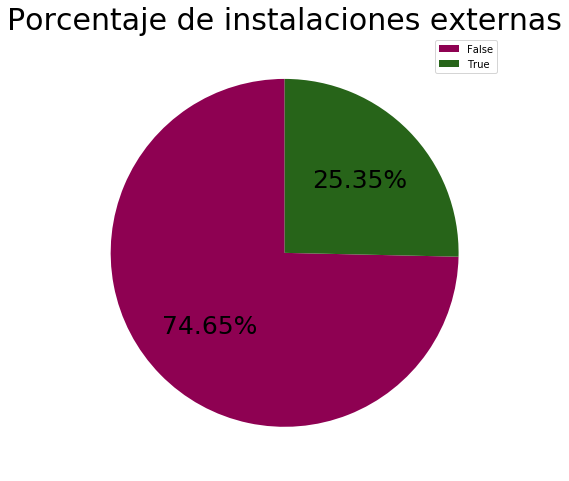
\includegraphics[width=300pt]{images/installs/implicit.png}
			\caption{Porcentaje de instalaciones atribuidas a la competencia}
		\end{figure}
		\FloatBarrier
		
		Los datos muestran un \textit{ratio} de algo más de 1 de cada 4 instalaciones atribuidas a empresas rivales.
		
		Si lo trasladamos nuevamente a las 5 aplicaciones más instaladas.
		
		\FloatBarrier
		\begin{figure}[h]
			\centering
			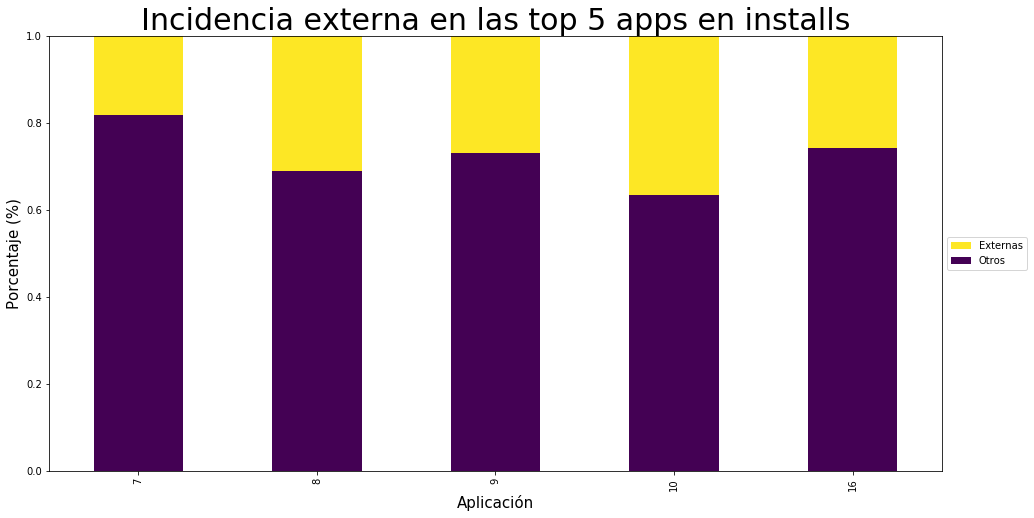
\includegraphics[width=\textwidth]{images/installs/incidenciacomp.png}
			\caption{Porcentaje de instalaciones atribuidas a la competencia para las top 5 apps en descargas}
		\end{figure}
		\FloatBarrier
		
		Como podemos ver, los resultados van acorde a lo mostrado en la figura anterior, con casos como el de la aplicación 10, donde casi el 40\% de las instalaciones le pertenecen a la competencia. Sin embargo, cabe destacar que en la aplicación líder en descargas, la cual supera a su perseguidora por más de 200 instalaciones (véase sección \ref{aplicaciones}), es donde las empresas rivales tienen menos presencia.
		
\section{Análisis de archivos en conjunto}

\section{Conclusion}


\bibliographystyle{plain}
\bibliography{references}
\end{document}
